\documentclass{article}

\usepackage{amsthm}
\usepackage{amsfonts}
\usepackage{amsmath}
\usepackage{amssymb}
\usepackage{fullpage}
\usepackage[usenames]{color}
\usepackage{hyperref}
  \hypersetup{
    colorlinks = true,
    urlcolor = blue,       % color of external links using \href
    linkcolor= blue,       % color of internal links 
    citecolor= blue,       % color of links to bibliography
    filecolor= blue,        % color of file links
    }

\usepackage{listings}
\usepackage{graphicx}
\graphicspath{ {./Report Images/} }

\definecolor{dkgreen}{rgb}{0,0.6,0}
\definecolor{gray}{rgb}{0.5,0.5,0.5}
\definecolor{mauve}{rgb}{0.58,0,0.82}

\lstset{frame=tb,
  language=haskell,
  aboveskip=3mm,
  belowskip=3mm,
  showstringspaces=false,
  columns=flexible,
  basicstyle={\small\ttfamily},
  numbers=none,
  numberstyle=\tiny\color{gray},
  keywordstyle=\color{blue},
  commentstyle=\color{dkgreen},
  stringstyle=\color{mauve},
  breaklines=true,
  breakatwhitespace=true,
  tabsize=3
}

\theoremstyle{theorem} 
   \newtheorem{theorem}{Theorem}[section]
   \newtheorem{corollary}[theorem]{Corollary}
   \newtheorem{lemma}[theorem]{Lemma}
   \newtheorem{proposition}[theorem]{Proposition}
\theoremstyle{definition}
   \newtheorem{definition}[theorem]{Definition}
   \newtheorem{example}[theorem]{Example}
\theoremstyle{remark}    
  \newtheorem{remark}[theorem]{Remark}


\title{CPSC-406 Report}
\author{Marc Nathaniel Domingo  \\ Chapman University}

\date{\today}

\begin{document}

\maketitle

\begin{abstract}
The purpose of this course is to understand how the Theory of Algorithms coincide with the application of functions and algorithms in Software Engineering. In particular, this course places an emphasis on the concepts of Automata, Logic, and Concurrency in regard to algorithms in our eventual application of these topics to a final project. 
\end{abstract}

\tableofcontents

\section{Introduction}\label{intro}
\subsection{Week 1} During this week, the overall outline and "roadmap" of topics and project deadlines were covered during class, as well as an introduction to the concept of Definitive Finite Automata (DFA).
\subsection{Week 2} Lectures covered Definitive Finite Automata (DFA) and Non-Definitive Finite Automata (NFA) in more detail, as well as how to convert NFA to DFA.
\subsection{Week 3} During this week, the lectures covered the concepts of querying a database, as well as algorithms for Unification and Resolution.
\subsection{Week 4} During this week, lectures covered the concept of Distributed Hash Tables (DHT) in the application of Decentralized Systems.
\subsection{Week 5} During this week, the lectures covered the concepts of Turing Machines and their relation to Polynomial and Non-Polynomial Time Problems.
\subsection{Week 6} During this week, the lectures reviewed Satisfiability as covered during our lectures on Non-Polynomial Time Problems in their application to a Sudoku Solver.
\subsection{Week 7} During this week, the lectures covered the concept of Distributed Systems in terms of how to create a Logical Clock.
\subsection{Week 8} During this week, the lectures covered the concept of Big O-complexity in terms of certain sorting algorithms such as bubble sort, in addition to an introduction to Complexity Theory.
\subsection{Week 9} During this week, the lectures covered the concept of model checking in addition to how the Needham-Schroeder Key Protocol can be modeled through Spin to witness how messages can be intercepted.
\subsection{Week 10} During this week, the lectures covered the concept of Temporal Logic and how it can be applied to solve Satisfiability problems.
\subsection{Week 11} During this week, the lectures covered the concepts of Composing Automata in addition to writing Regular Expressions based off of Non-Definitive Automata (NFA).
\subsection{Week 12} During this week, the lectures covered the concepts of Atomicity, Sequential Consistency, and Weak Memory in the context of a multi-threaded program in addition to what Safetiness, Liveliness, and Fairness are defined as within the context of a system.
\section{Homework}\label{homework}

This section contains solutions to homework. 

\subsection{Week 2}
The objective of this week's homework is to convert a given NFA to a DFA by hand.
\\ 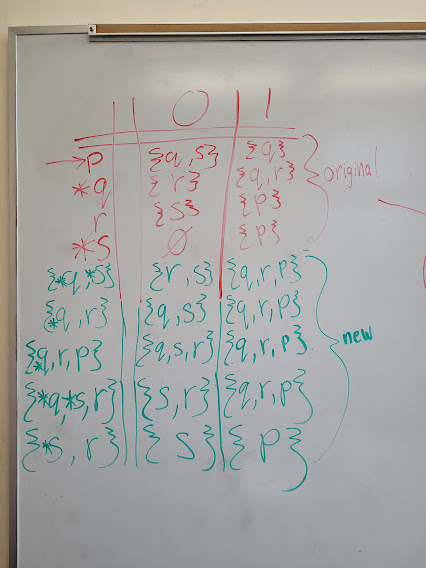
\includegraphics[width=15cm, height=8cm]{Report Images/HW2_1.jpg}
\\ 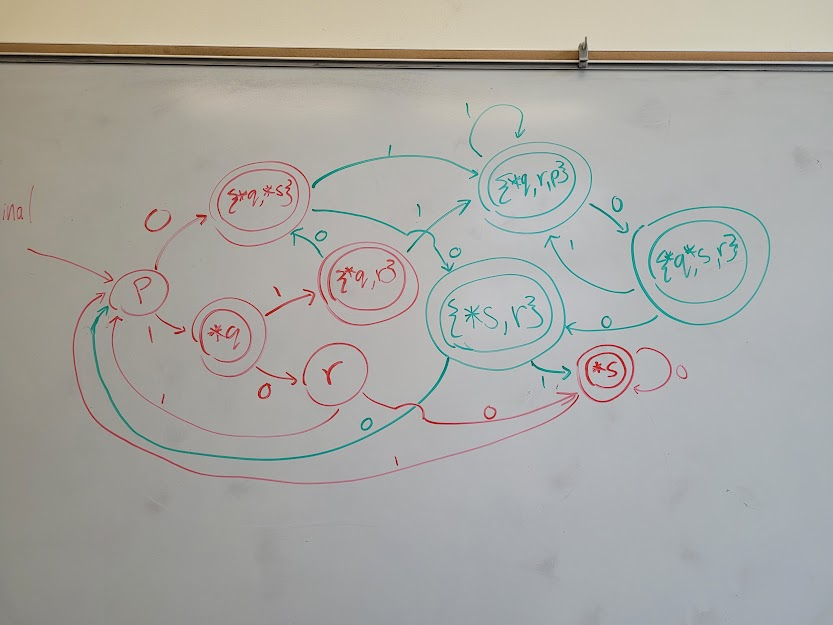
\includegraphics[width=15cm, height=8cm]{Report Images/HW2_2.jpg}
\subsection{Week 3}
The objective of this week's homework is to solve Unification Algorithm problems in addition to practicing drawing an SLD-tree solution to a program given a particular input.
\\ 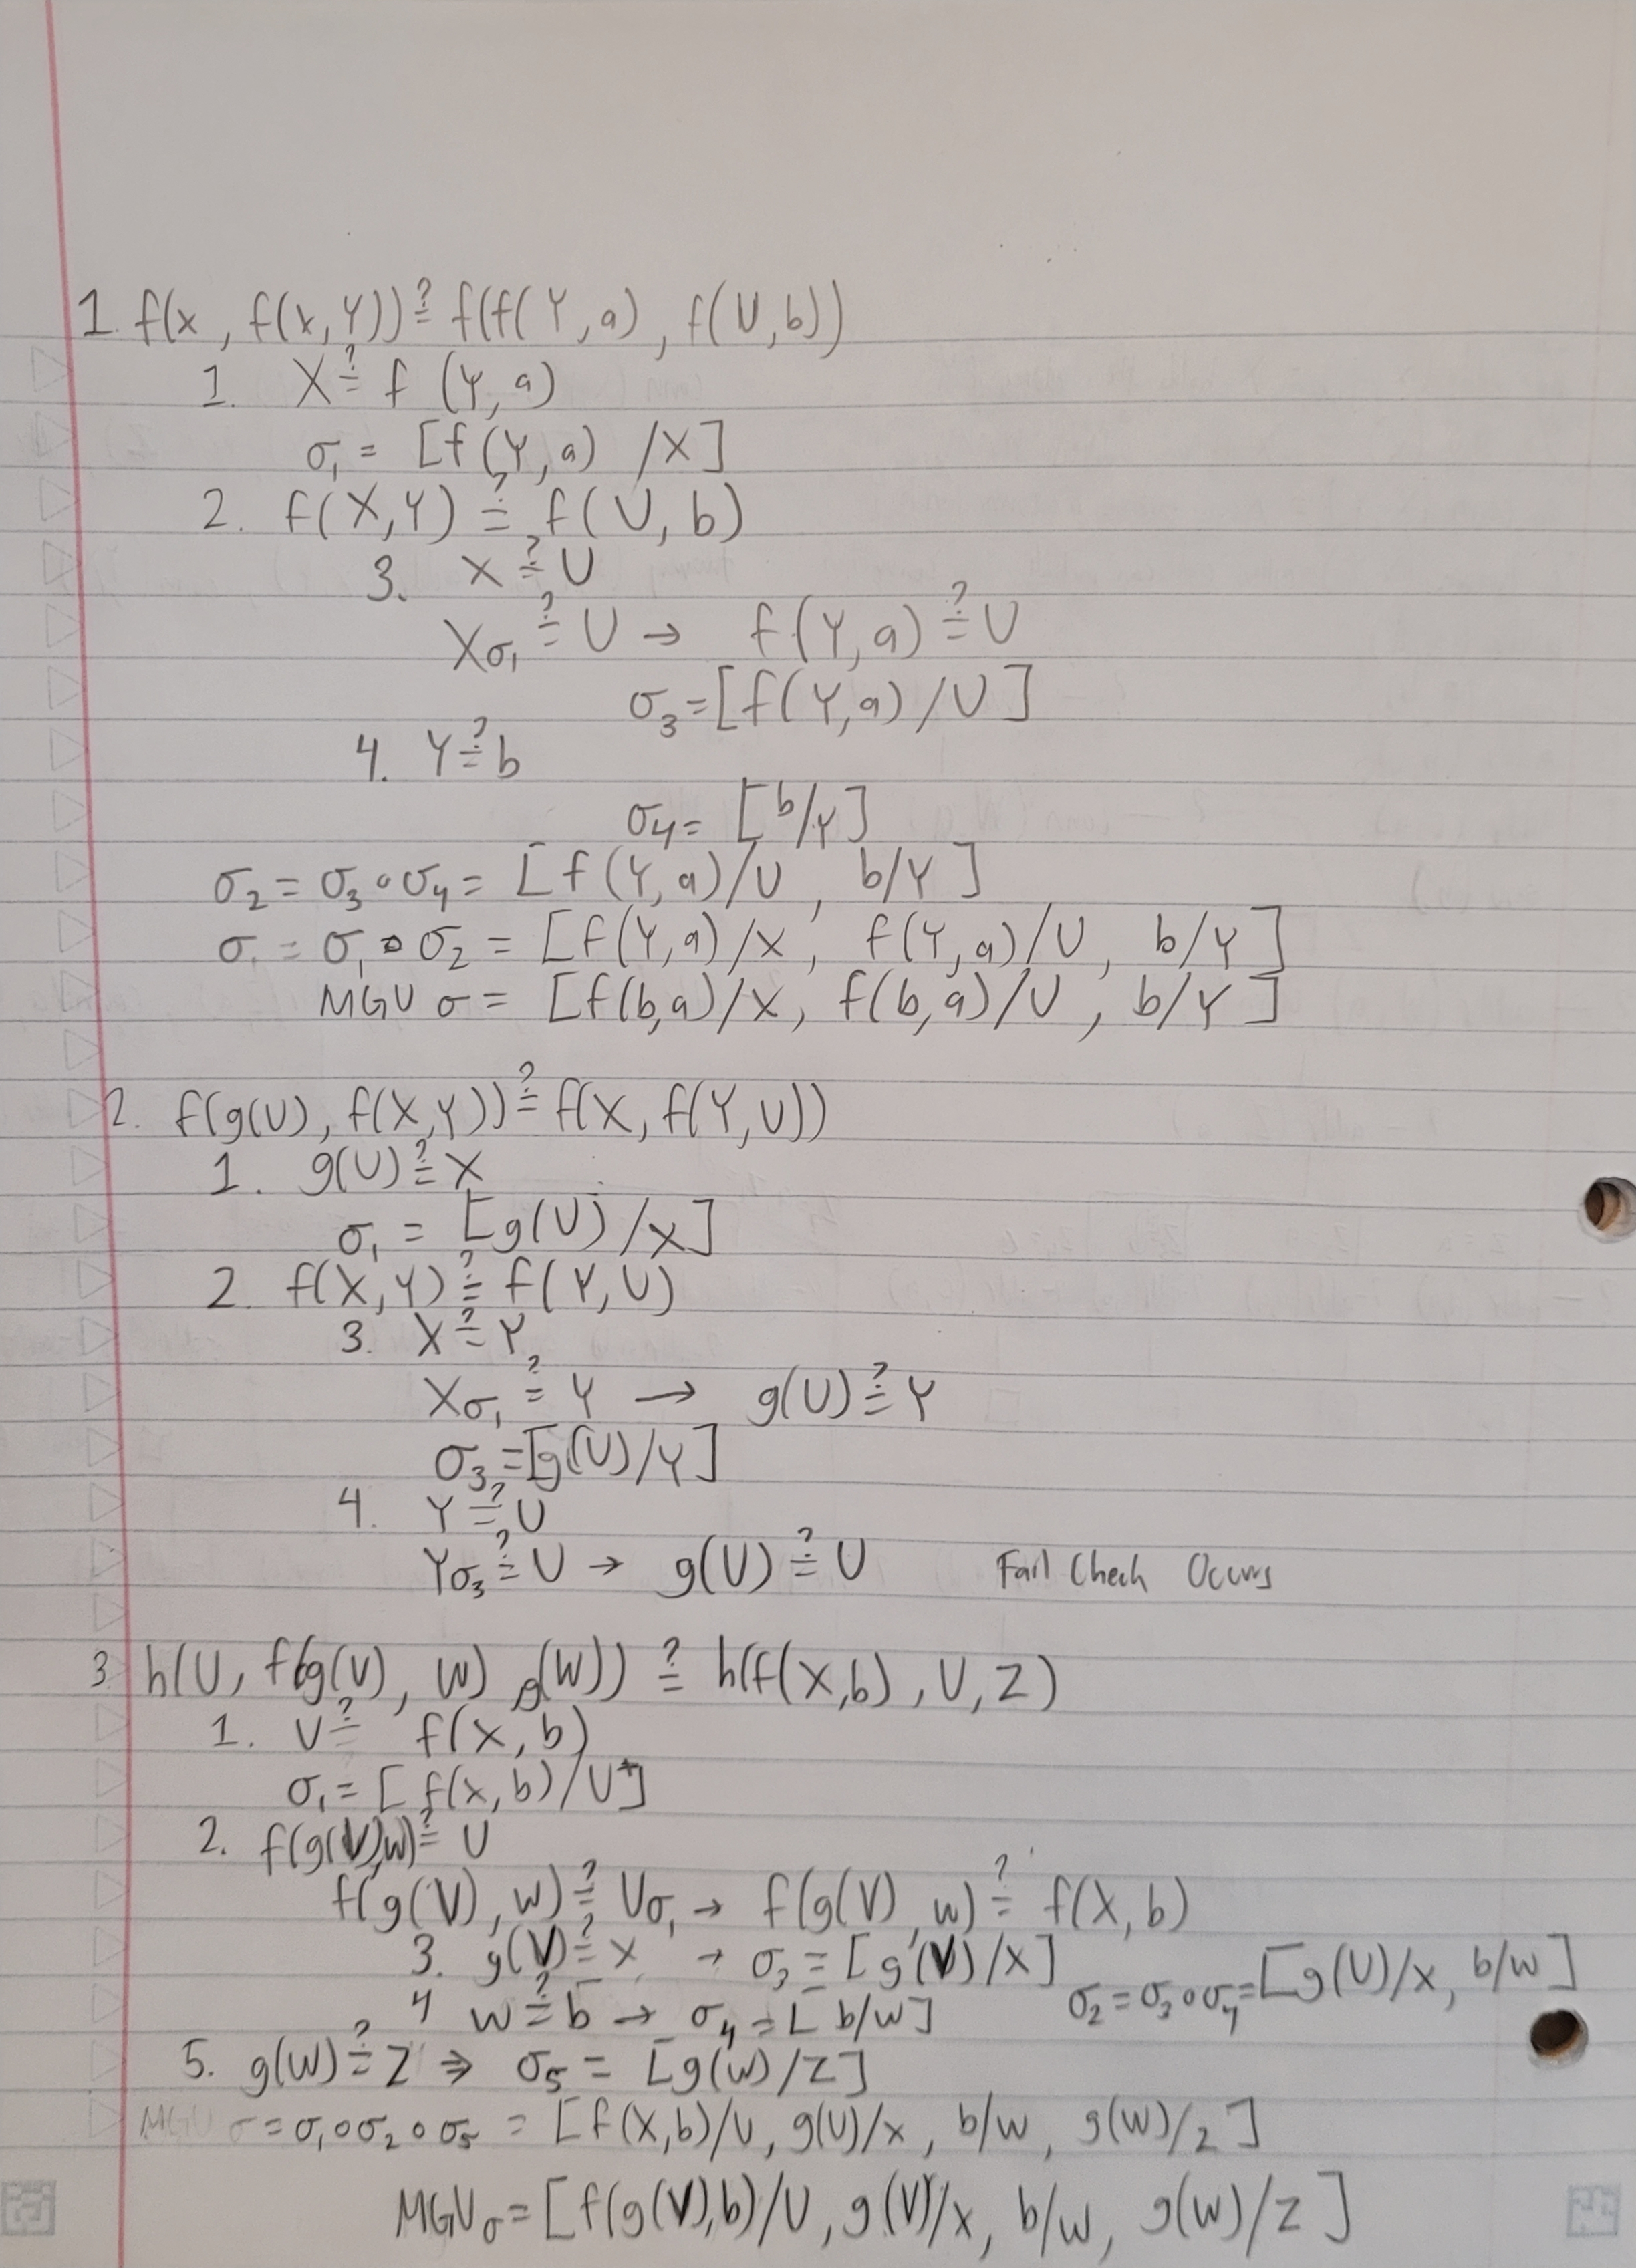
\includegraphics[width=18cm, height=20cm]{Report Images/HW3_1.jpg}
\\ 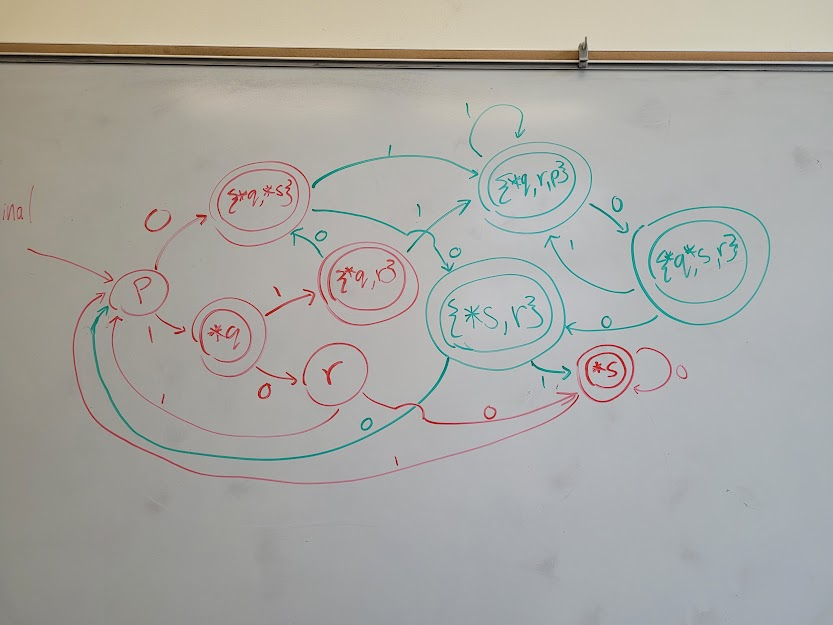
\includegraphics[width=18cm, height=20cm]{Report Images/HW3_2.jpg}
\subsection{Week 6}
The objective of this week's homework was to create Indirect Truth Tables to understand Satisfiability in terms of Propositional Logic. For the following tables, we used the Indirect Truth Table method to prove why the formulas above the tables are valid.
\\ 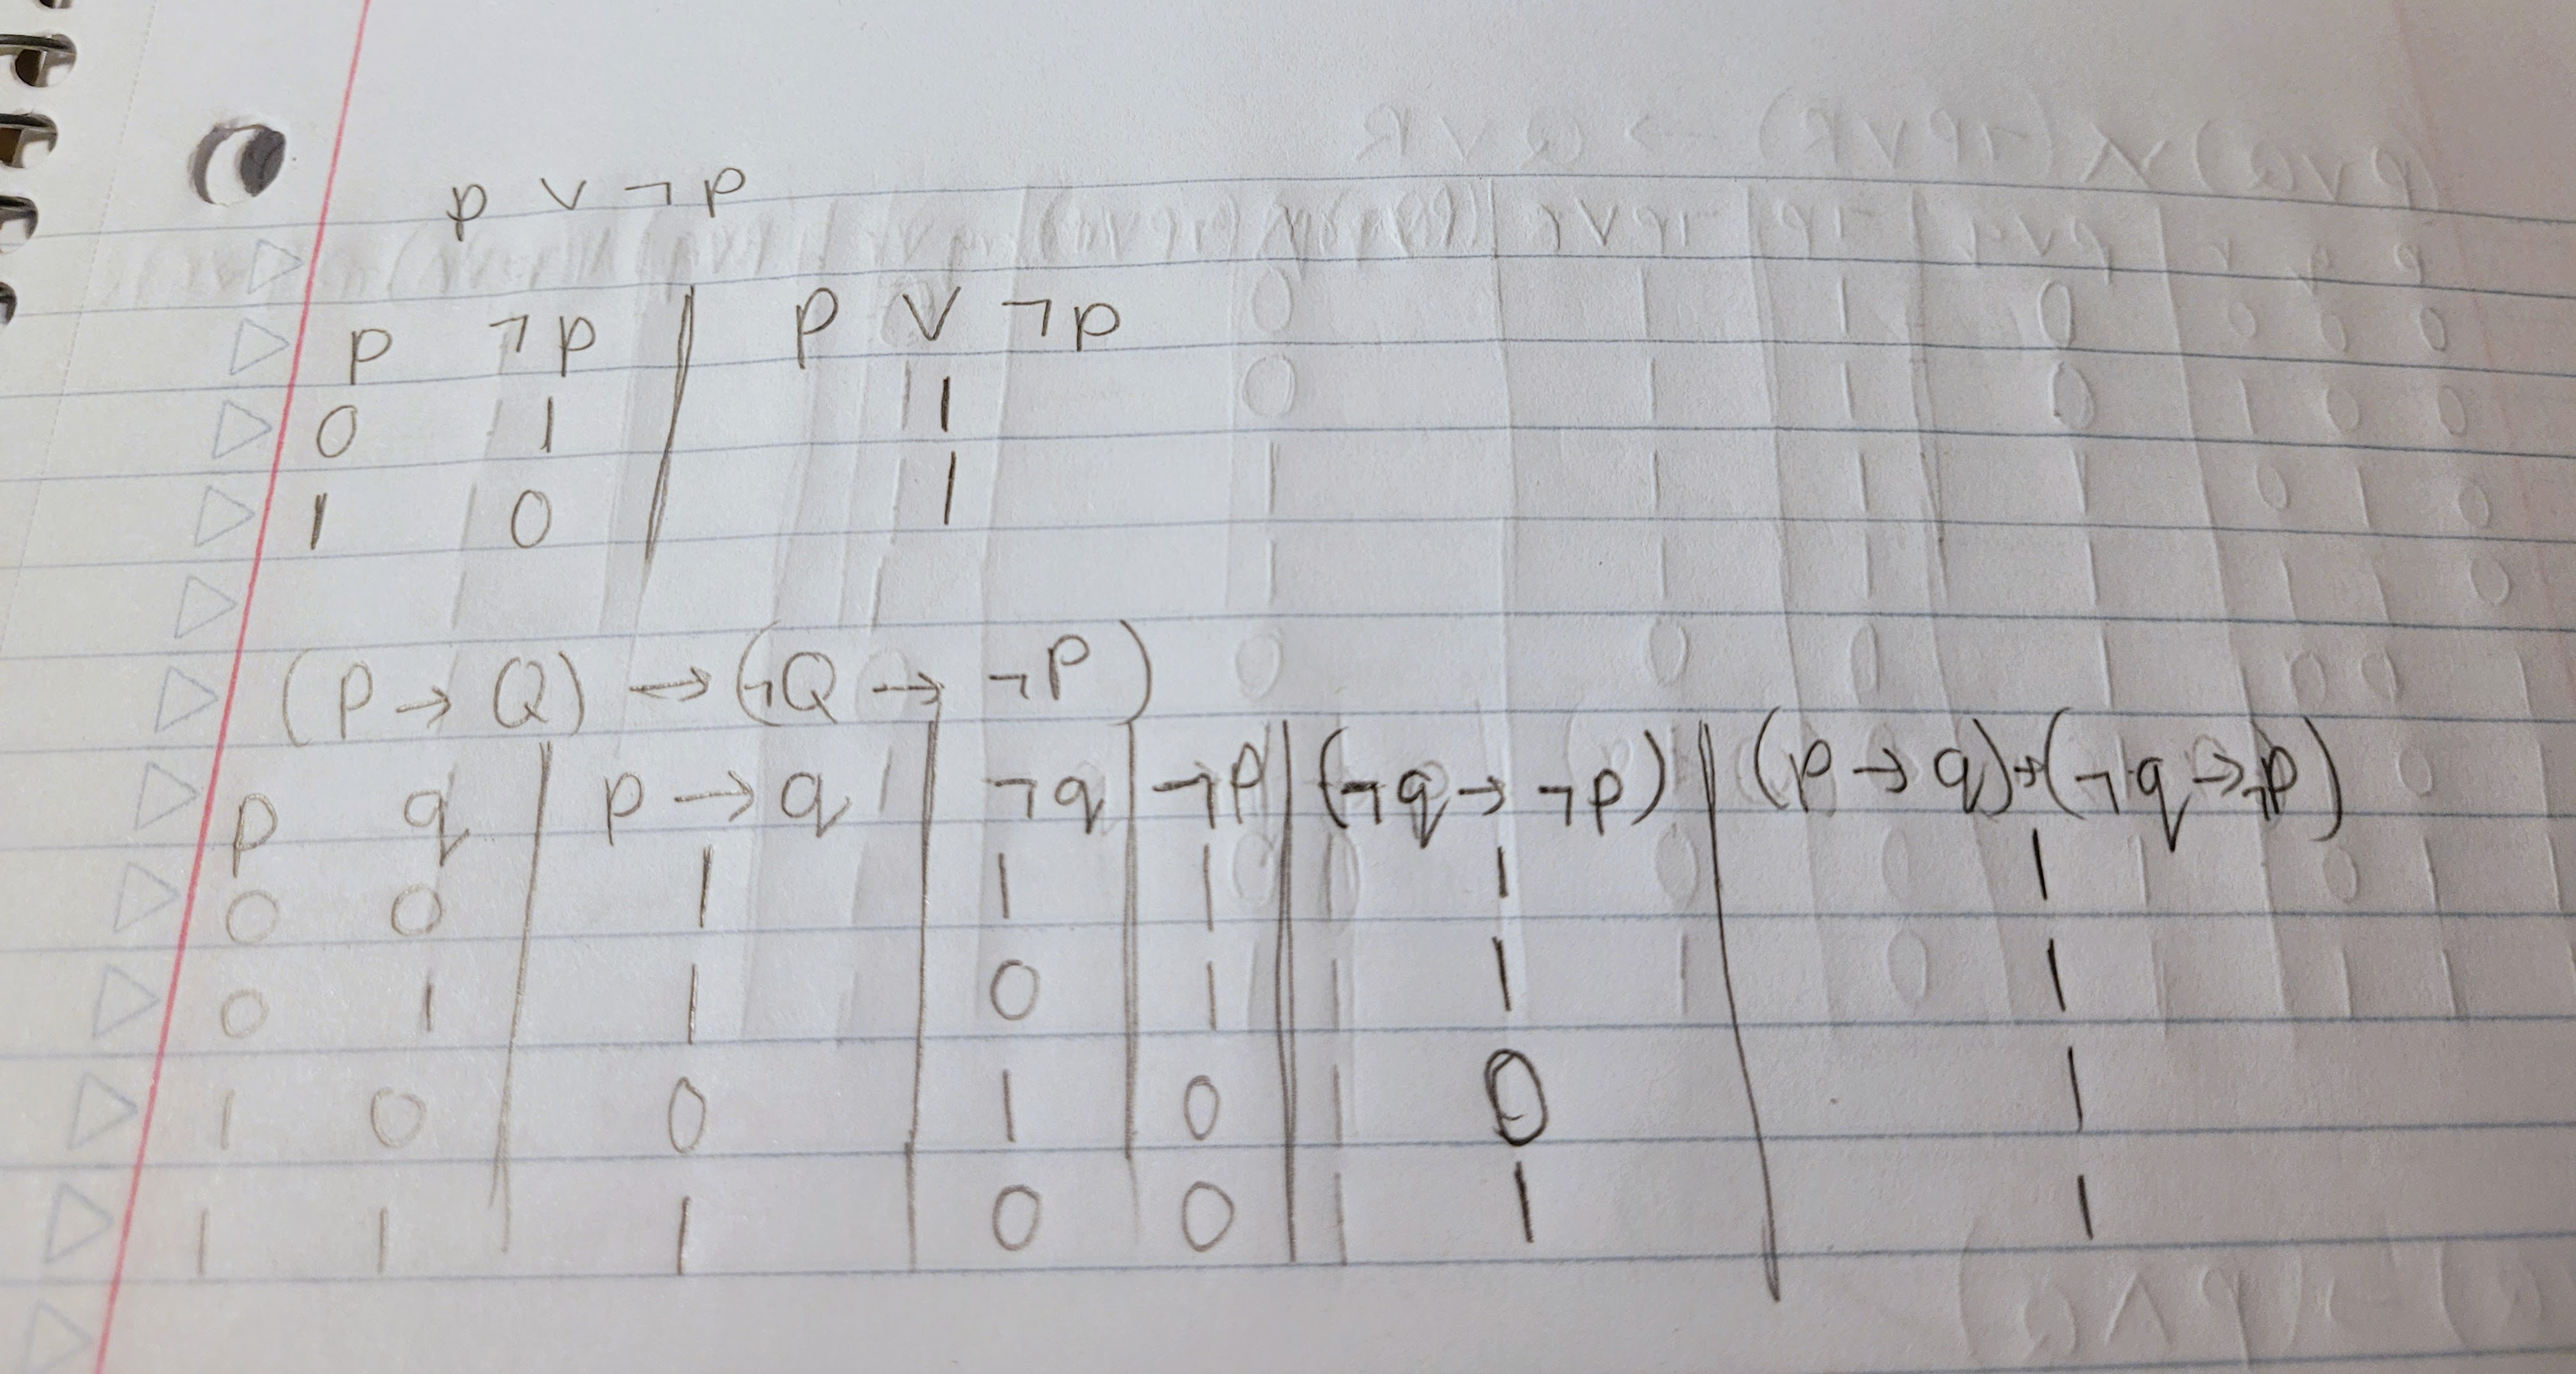
\includegraphics[width=15cm, height=8cm]{Report Images/HW6_1.jpg}
\\ 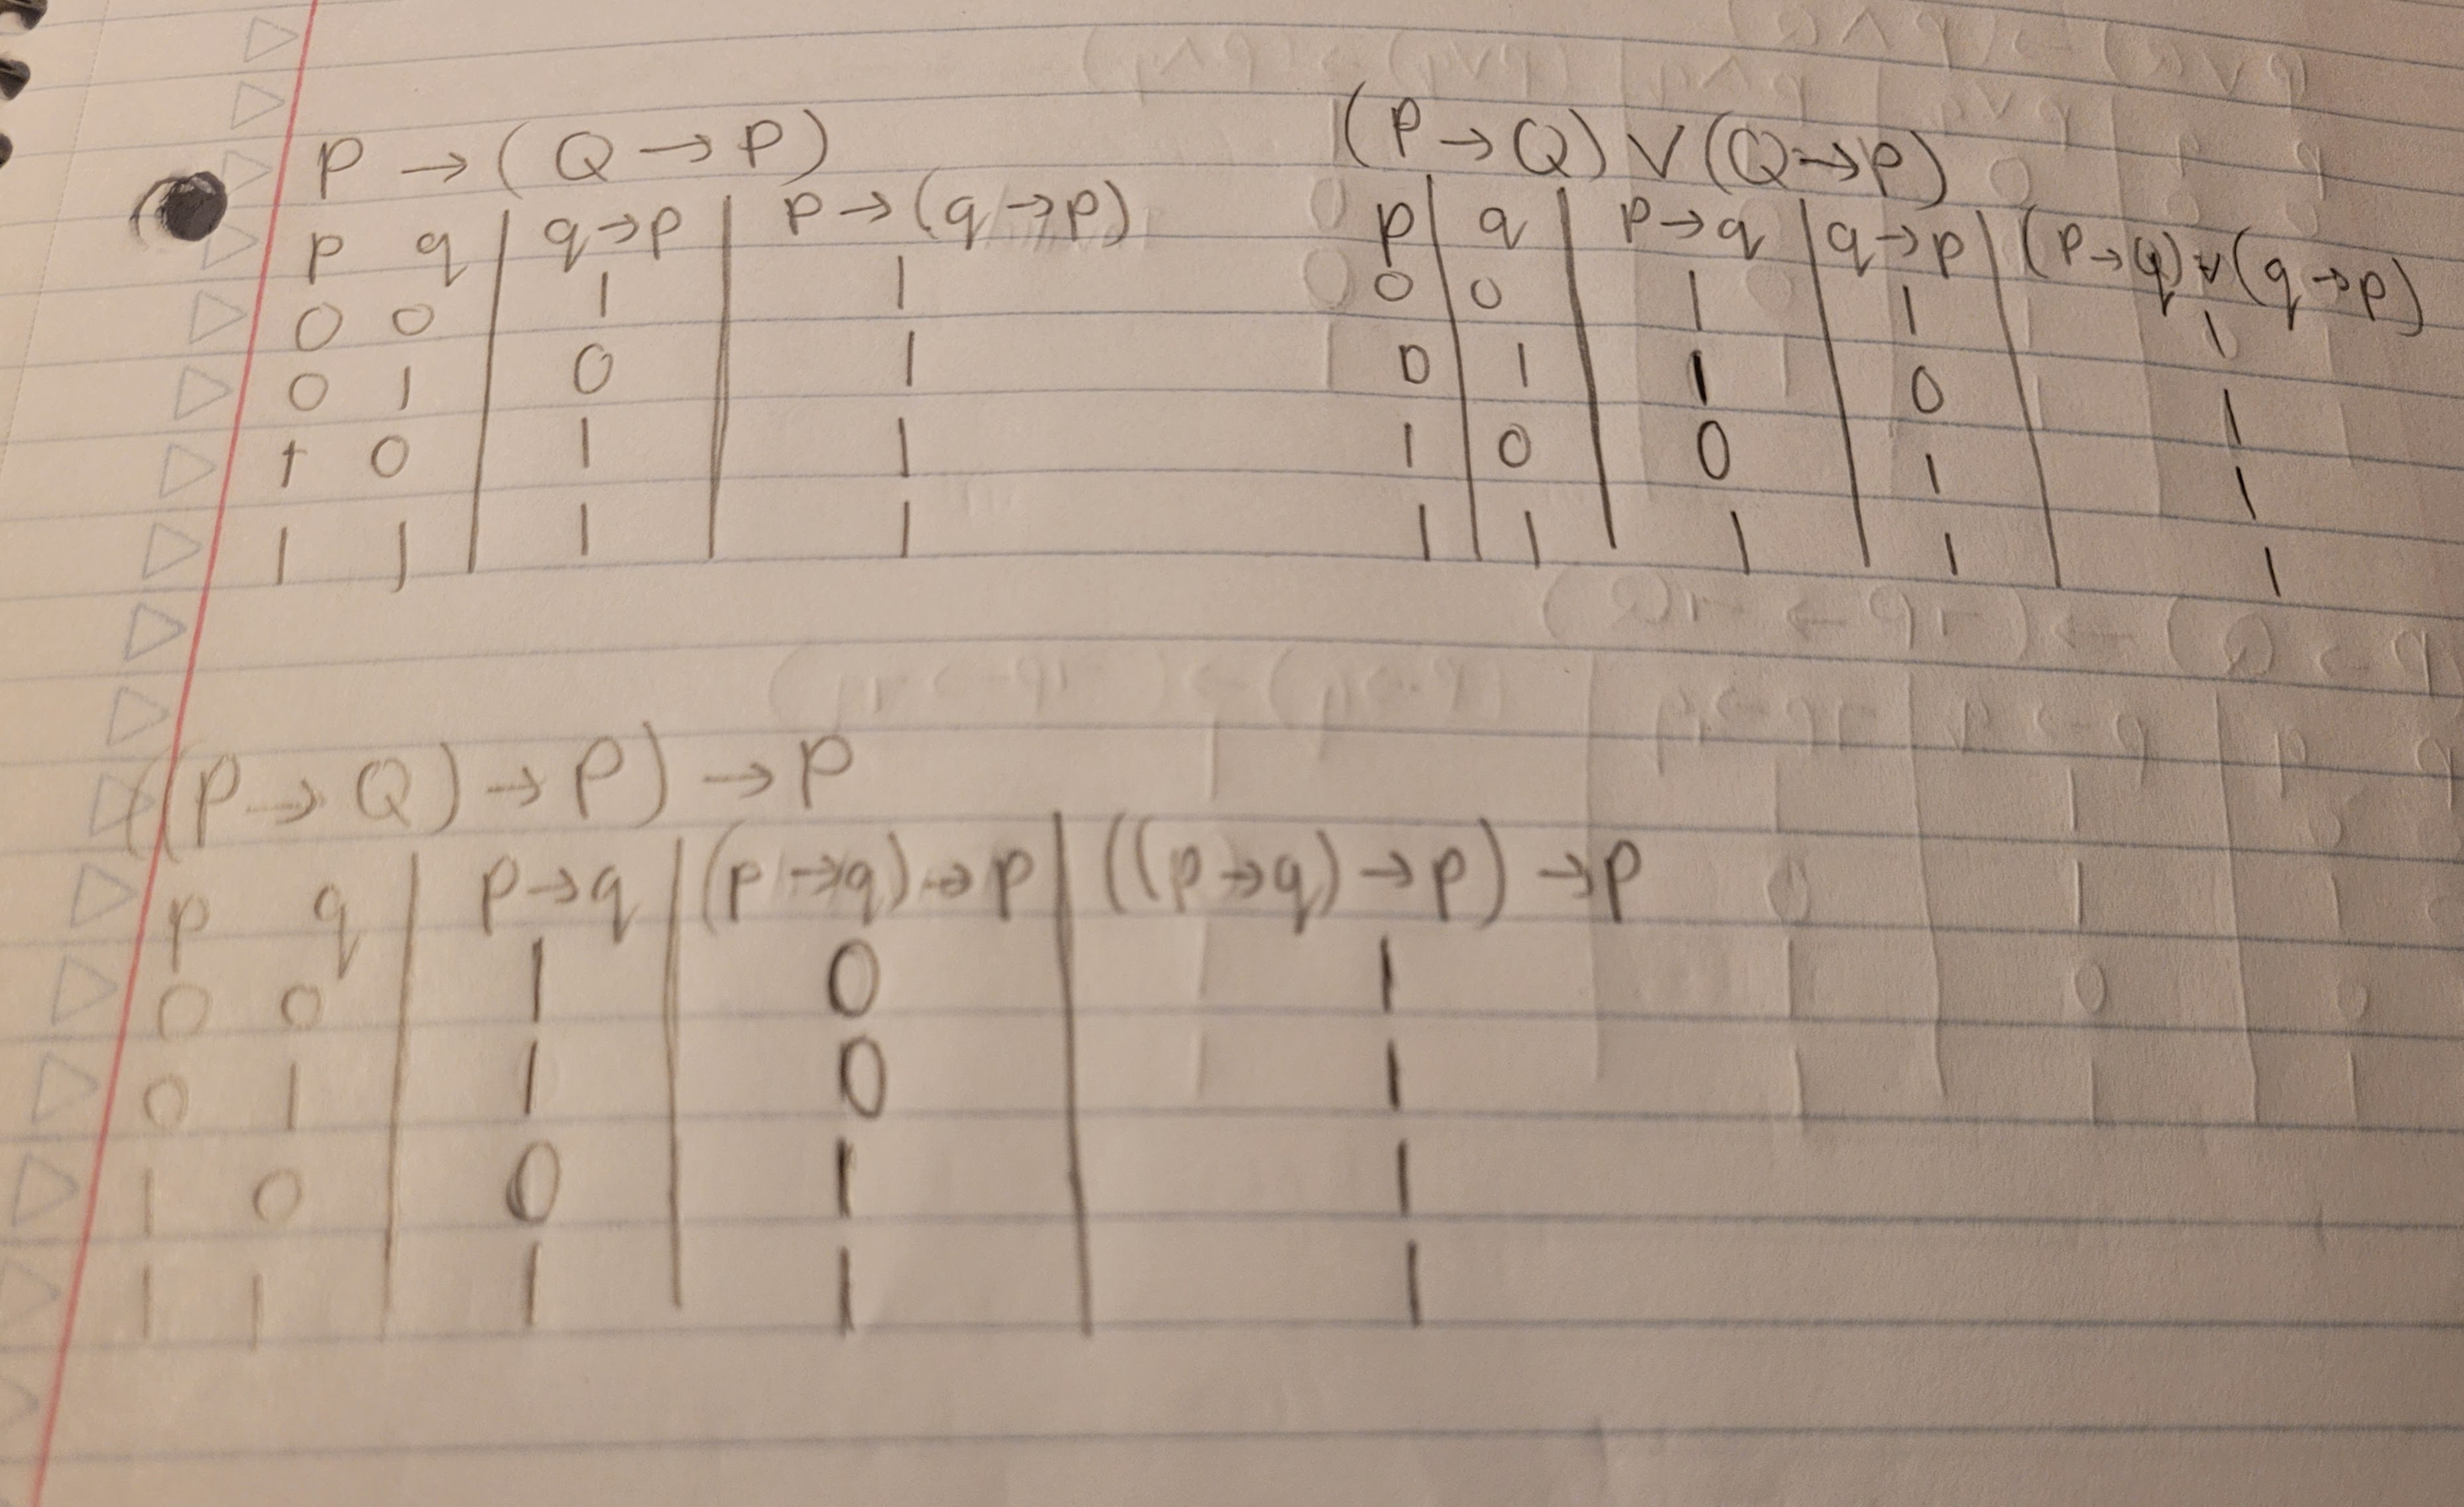
\includegraphics[width=15cm, height=8cm]{Report Images/HW6_2.jpg}
\\ 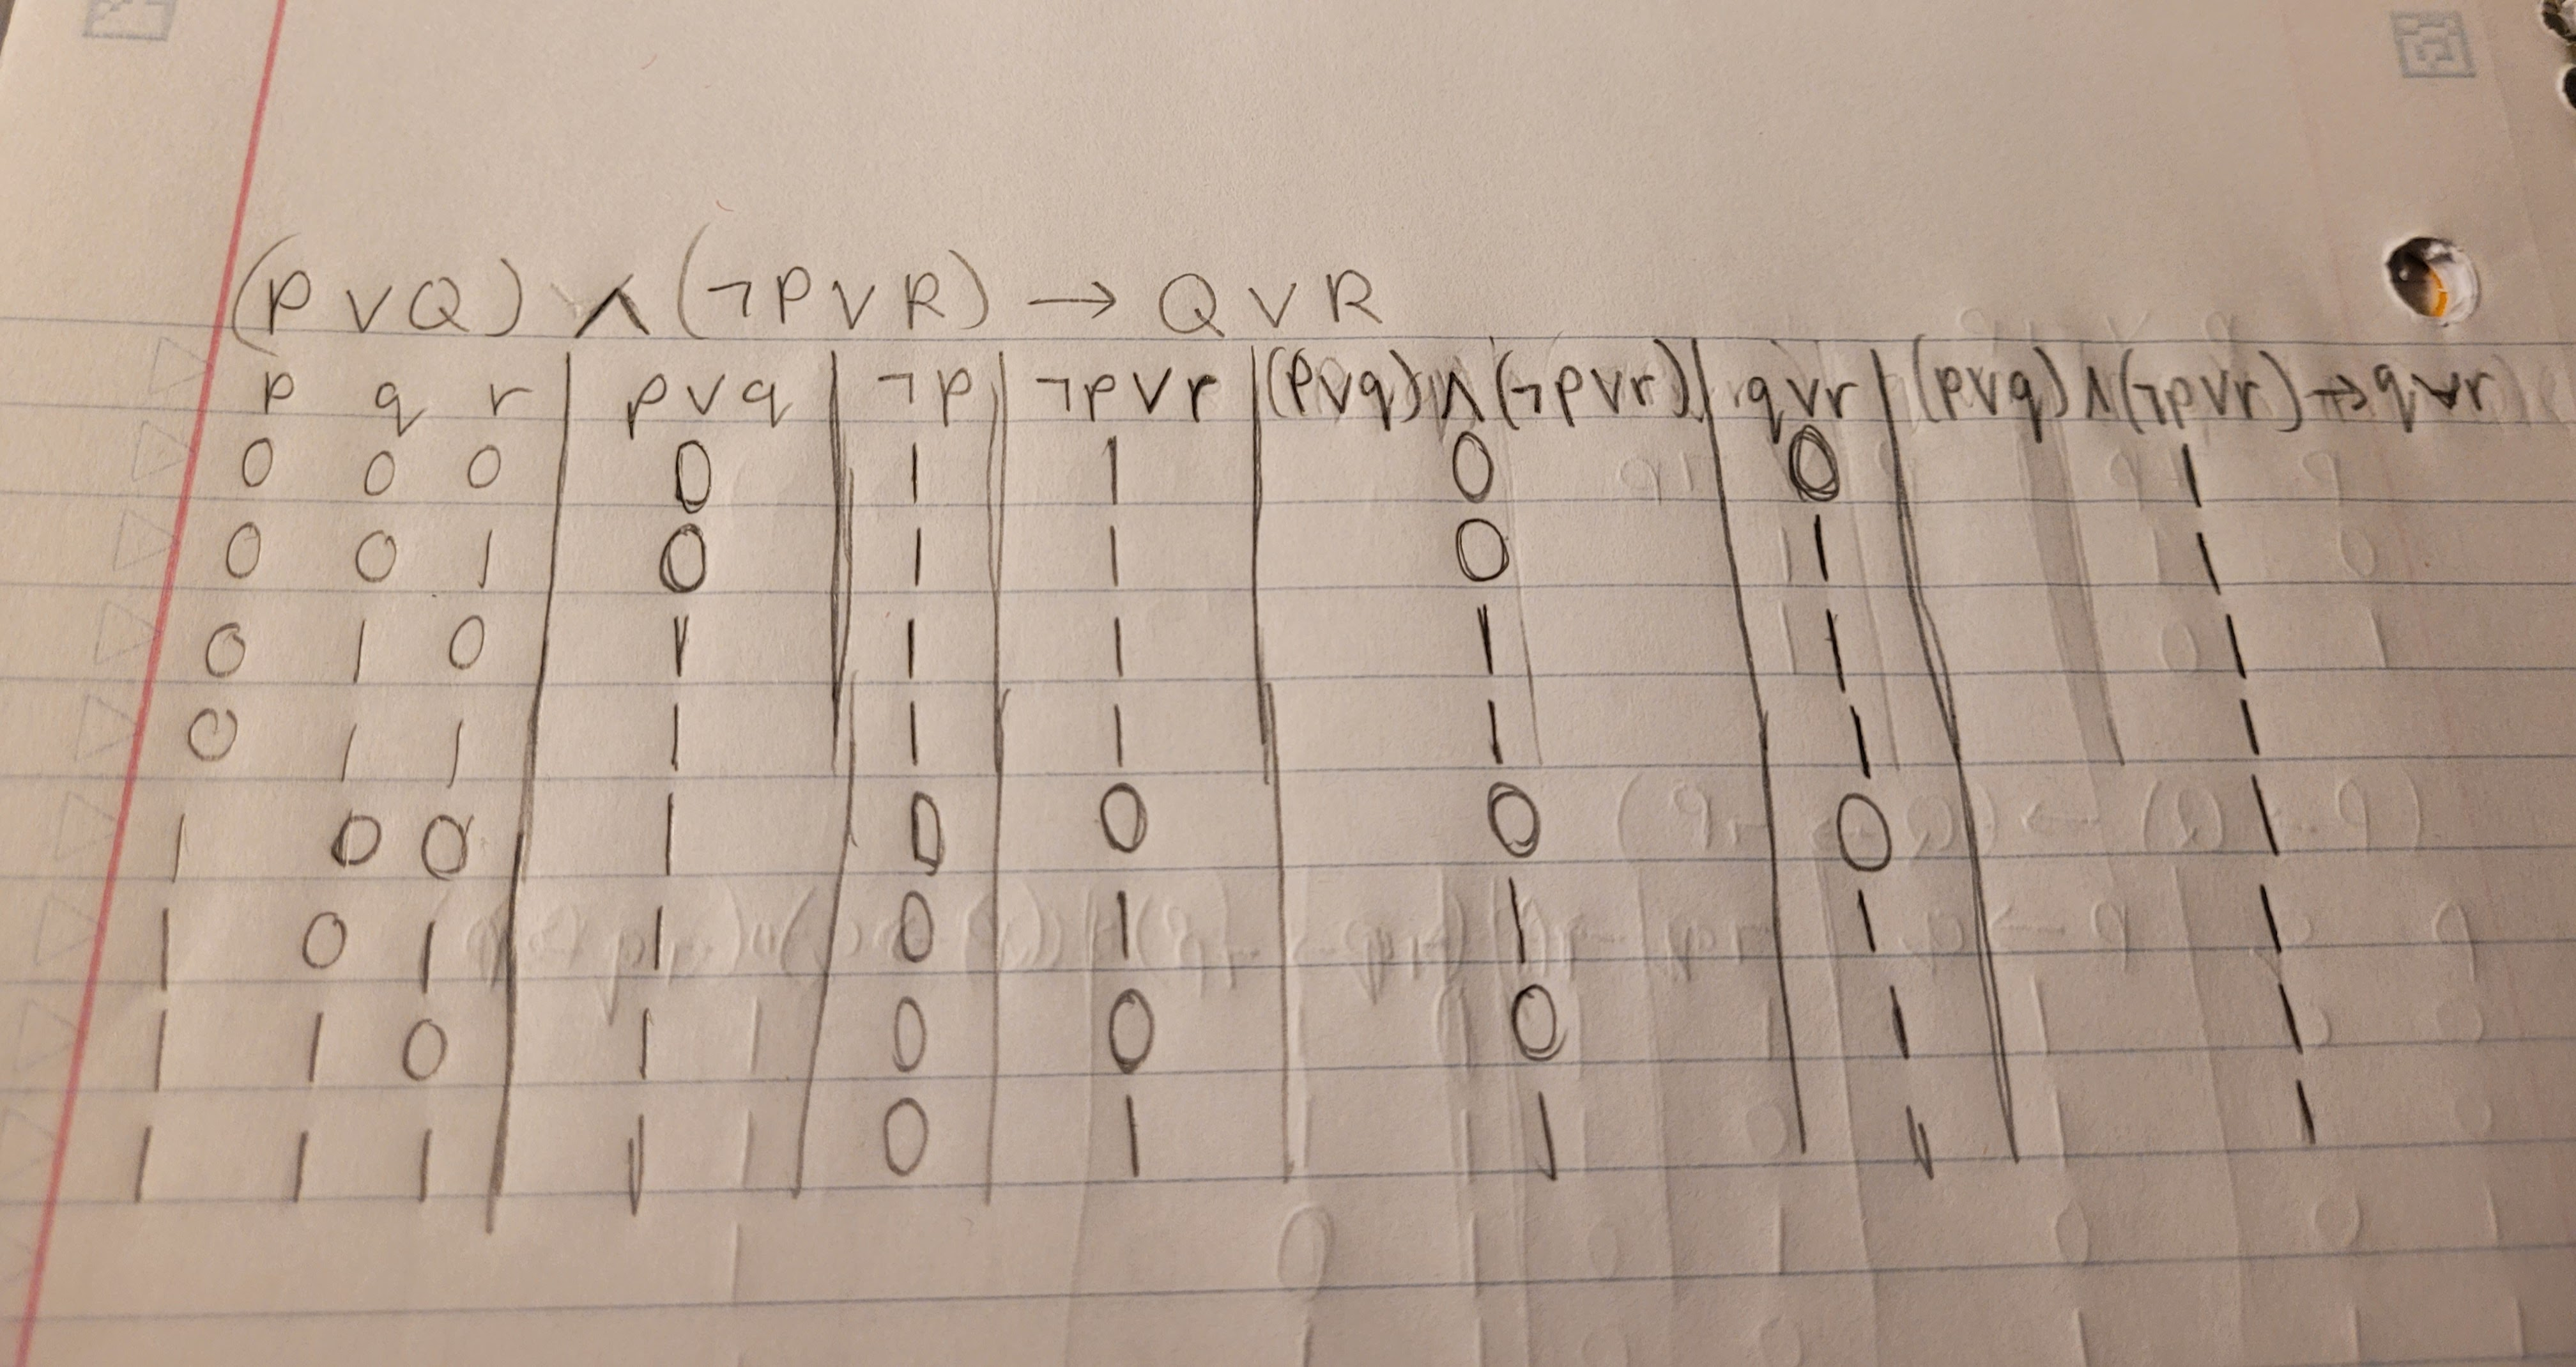
\includegraphics[width=15cm, height=8cm]{Report Images/HW6_3.jpg}
\\
For the following tables, the Indirect Truth Table method was used to prove why the formulas above the table are not valid.
\\ 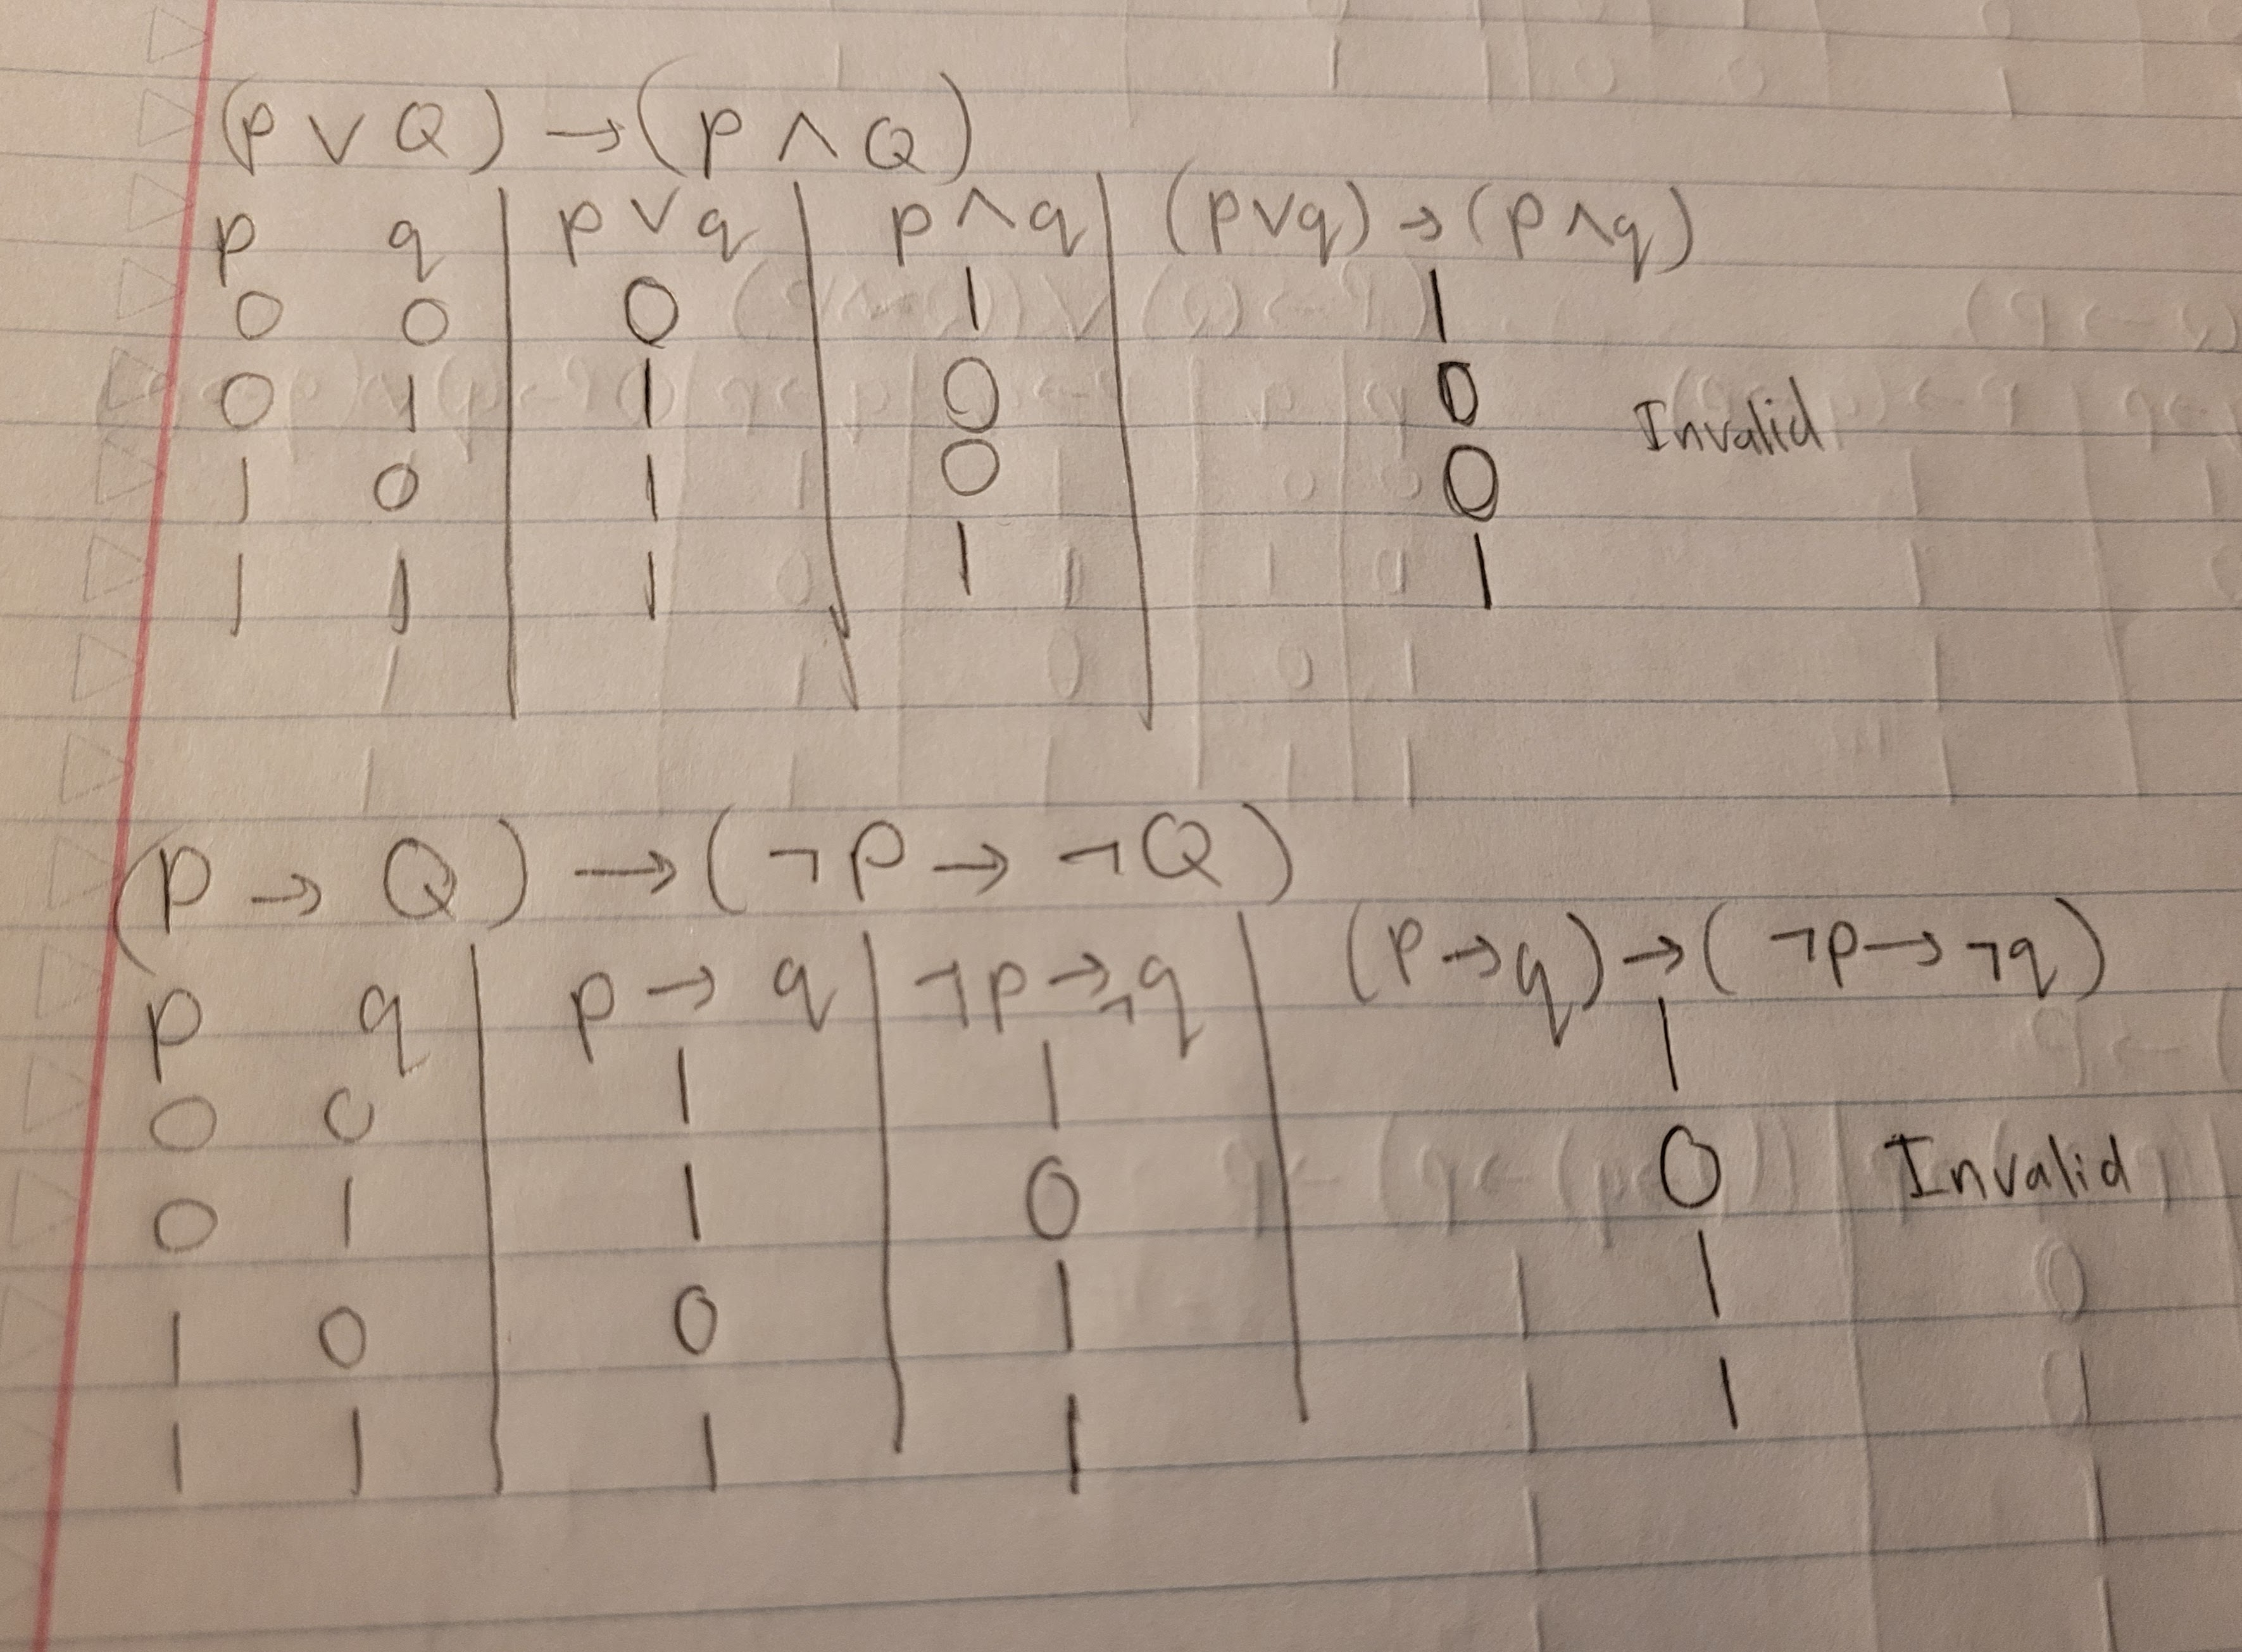
\includegraphics[width=15cm, height=8cm]{Report Images/HW6_4.jpg}
\subsection{Week 9}
The objective of this week's homework is to explore exercises relating to the Needham-Schroeder Public-Key Protocol using Spin models.
\\
\\ One such example is to go through the program \textbf{ns.pml} and define what the meaning behind the propositions \textit{success}, \textit{AliceBob}, and \textit{BobAlice}.
\begin{itemize}
\item \textbf{success} is a propositional variable that is true if and only if the first protocol (Alice) has successfully sent a reply to the second protocol (Bob), and if the second protocol (Bob) had sent a reply to the first protocol's (Alice) initial message.
\item \textbf{aliceBob} is a propositional variable that is true if and only if the partner of the first protocol, Alice, is Bob.
\item \textbf{bobAlice} is a propositional variable that is true if and only if the partner of the second protocol, Bob, is Alice.
\end{itemize}
The next exercise required determining which of the two formulas at the bottom of the code would violate the protocol when executed, as well as to explain the nature of the protocol based on that violation. \\
\begin{itemize}
    \item The violation was caused by $$ltl \{[]  (success \&\& aliceBob \xrightarrow{} aliceBob)\}$$
    \item As the only difference between the two lines is the placement of \textbf{aliceBob} and \textbf{bobAlice} are swapped, this implies that the protocol is hard-coded such that the protocol does not get violated if Alice replies to Bob's reply, but in the event that the roles are reversed, the protocol is susceptible to intruders.
\end{itemize}
The next exercise of the homework involved looking through the execution sequence output from the protocol violation.
\begin{itemize}
    \item The execution sequence ended up being 83 lines long, which matched up with the protocol violation message, with an additional line representing the attempt at the next check.
\end{itemize}
The last exercise involved creating a Message Sequence Chart (MSC) that represents a successful attack on the protocol.
\\ 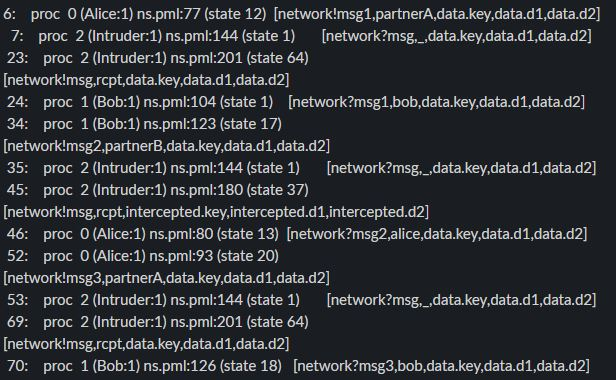
\includegraphics{Report Images/HW9_1.jpg}
\begin{itemize}
    \item The MSC represents a successful attack on the protocol as the intruder has managed to message both Alice and Bob before the other is able to receive and reply to the message from a proper protocol.
\end{itemize}
\subsection{Week 11}
The objective of this week's homework was to explore $\epsilon $-transitions and operations on various automata.
\\ 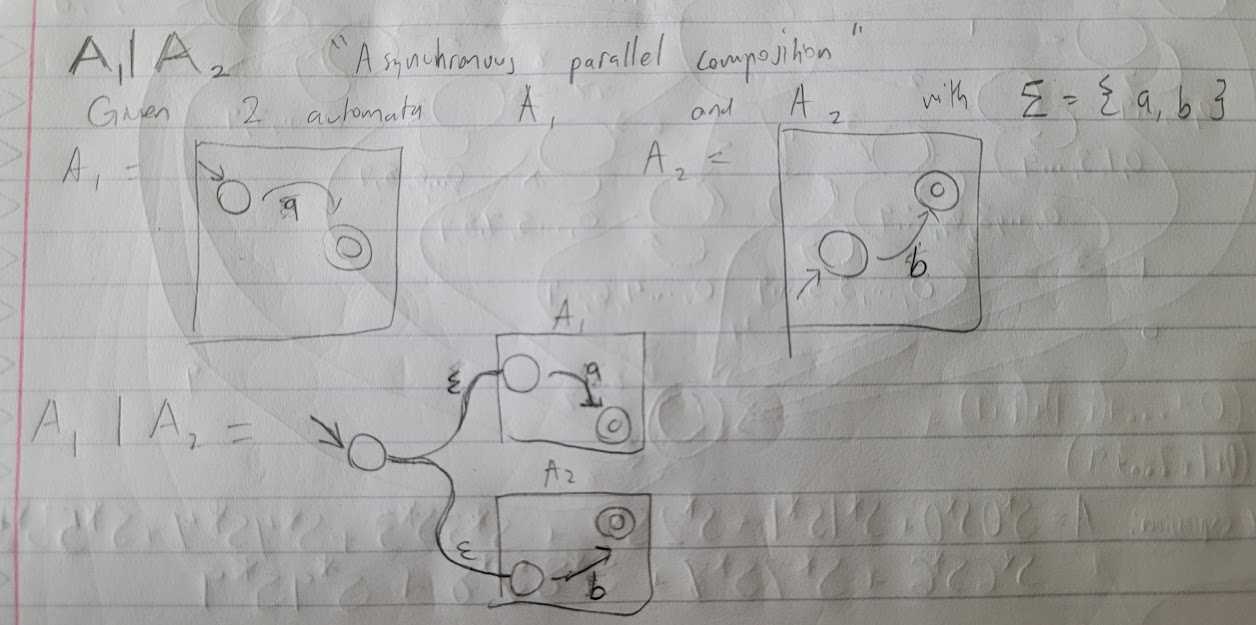
\includegraphics[width=15cm, height=8cm]{Report Images/HW11_1.jpg}
\begin{itemize}
    \item Asynchronous Parallel Composition accepts languages that are capable of operating in parallel to each other, utilizing a set of strings that consists of the combined alphabet that each language accepts.
    \item The above example would have a regular expression of $A_{1} | A_{2} = \epsilon a + \epsilon b $
\end{itemize}
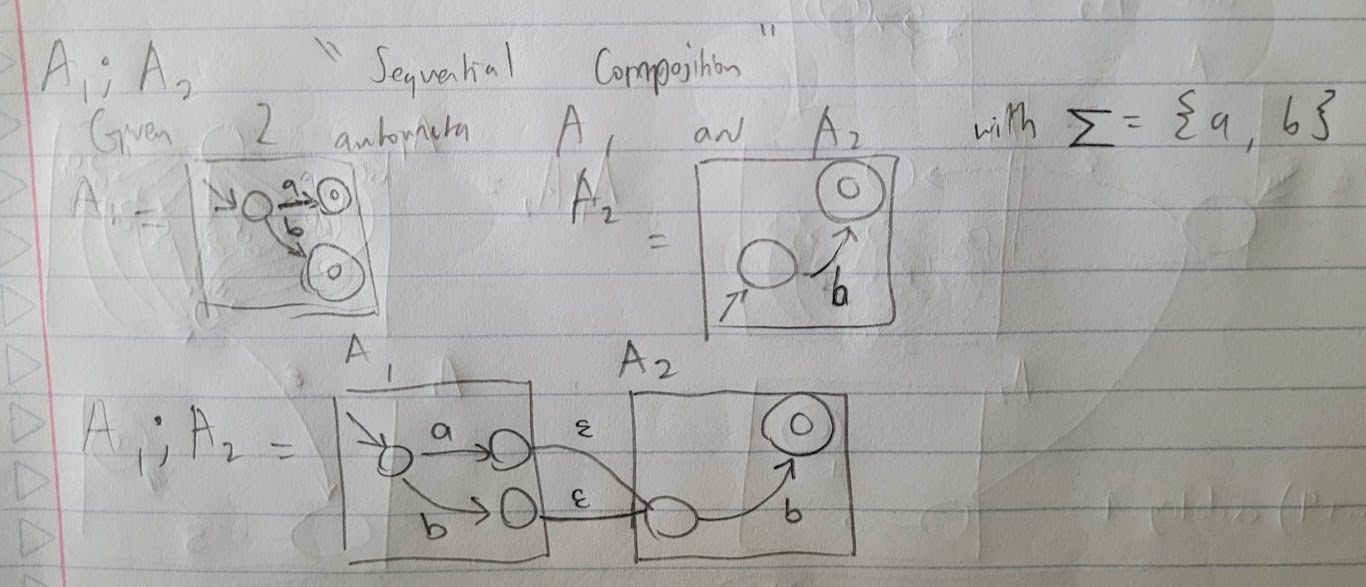
\includegraphics[width=15cm, height=8cm]{Report Images/HW11_2.jpg}
\begin{itemize}
    \item Sequential Composition accepts languages that are capable of running in a sequential sequence, that is the output of one language is used as the starting point of another language, utilizing a set of strings that both languages share.
    \item The above example would have a regular expression of $A_{1} ; A_{2} = (a+b)\epsilon b$
\end{itemize}
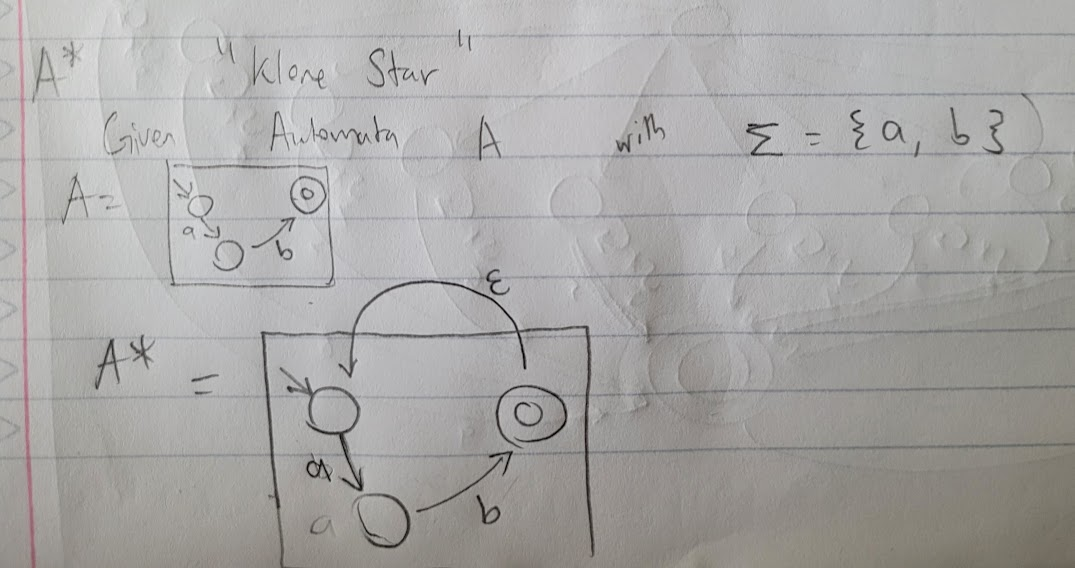
\includegraphics[width=15cm, height=8cm]{Report Images/HW11_3.jpg}
\begin{itemize}
    \item Kleene Star accepts languages that are capable of infinitely repeating, starting back at the machine's initial state.
    \item The above example would have a regular expression of $A^{*} = ab\epsilon^{*}$
\end{itemize}
The next section of the homework consisted of finding the DFA and regular expressions of examples from the textbook, as well as finding the $\epsilon$-NFA if the above operations were applied to the examples.
\begin{itemize}
    \item The set of strings over the alphabet \{ 0, 1, ... 9 \} such that the digit has appeared before.
\end{itemize}
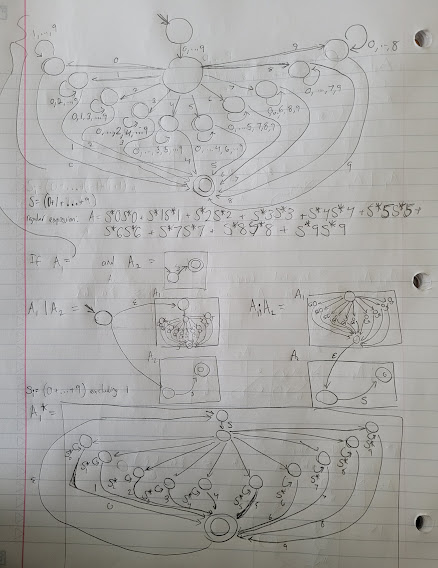
\includegraphics{Report Images/HW11_4.jpg}
\begin{itemize}
    \item The set of strings consisting of zero or more a's followed by zero or more b's, followed by zero or more c's.
\end{itemize}
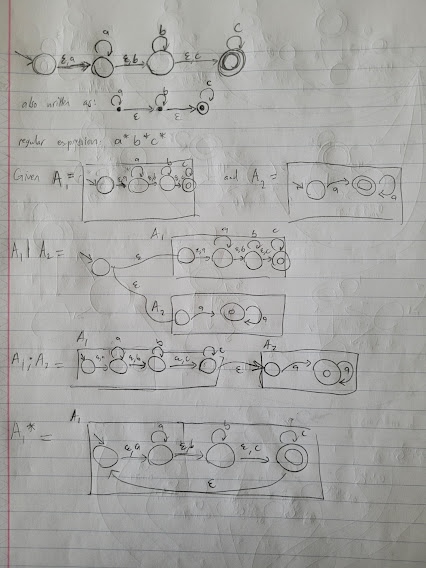
\includegraphics{Report Images/HW11_5.jpg}
\subsection{Week 12} The objective of this week's homework was to explore the concepts of Mutual Exclusion with and without Atomicity in addition to the concepts of Sequential Consistency in Weak Memory through the use of online multi-threading Java Programs. \\ 
\\ \textbf{Homework Question 1:} Have a look at \href{https://colab.research.google.com/drive/126wdCs8F_VJ7VwTcaXUv70PwAVTGzVy_?usp=sharing}{peterson.py}. What program behavior do you expect? Is your expectation confirmed when you run the program?
\begin{itemize}
    \item Based on the program itself, I expect the program to attempt to run both threads a total of 10000 times. The execution of each thread would iterate the "counter" of the program each time the thread is run, so I would expect the print statement at the end of the program to note that the program's counter ended at 20000. This expectation was confirmed after running the program.
\end{itemize}
\textbf{Homework Question 2:} Analyse the Java program \href{https://www.online-java.com/G0N5eA9tR6}{peterson} in the same way as you analysed the Python program in the previous exercise. Make sure to run the Java program on your local machine. What observations do you make?
\begin{itemize}
    \item Based on the program itself, I expect that the program, similar to the python program from the previous question, would attempt to run both threads a total of 10000 times as both the python and java programs share a similar code for what is defined as the "critical\textunderscore section" in the python file and what is defined as a "process" in the java file. During the execution of each thread, the program would iterate the "counter" variable after each thread has completed their process, and because both threads are running the "process" function that iterates 10000 times, I would expect the print statement at the end of the program to note that the counter ended at 10000. This expectation was confirmed after running the program.
    \item In terms of the program's behavior when executed, the java threading program appeared to run slower than the python program.
\end{itemize} 
\textbf{Homework Question 3:} Explain why the outcome \textbf{a} $=$ \textbf{0}, \textbf{b} $=$ \textbf{0} is not sequentially consistent, but the other three outcomes are.
\begin{itemize}
    \item The outcome \textbf{a} $=$ \textbf{0}, \textbf{b} $=$ \textbf{0} is not sequentially consistent within the context of the threading model as defined by \href{https://www.online-java.com/yFkZ4HqfRG}{memoryModel} as there exists no currently existing iteration within the program that would compute and read both \textbf{a} and \textbf{b} as \textbf{0} before they are overwritten by the values of \textbf{x} and \textbf{y}. Currently, getting both \textbf{a} and \textbf{b} as \textbf{0} could be possible without the resetting of all variables at the end of \textit{runTest()}.
\end{itemize}
\textbf{Homework Question 4:} Report the results you get from running \href{https://www.online-java.com/yFkZ4HqfRG}{memoryModelWithStats} on your local machine. Include the specs of your processor, in particular the number of cores. If you can find out something about the caches, add this as well.
\begin{itemize}
    \item Processor Information:
    \begin{itemize}
        \item Name: Intel(R) Core(TM) i5-7200U CPU @ 2.50GHz   2.71 GHz
        \item Base Speed: 2.71 GHz
        \item Number of Sockets: 1
        \item Number of Cores: 2
        \item L1 Cache: 128 KB
        \item L2 Cache: 512 KB
        \item L3 Cache: 3.0 MB
    \end{itemize}
    \item Results from \href{https://www.online-java.com/yFkZ4HqfRG}{memoryModelWithStats} :
    \begin{itemize}
        \item (0, 0): 0
        \item (0, 1): 538
        \item (1, 0): 461
        \item (1, 1): 1
    \end{itemize}
\end{itemize}
\textbf{Homework Question 5:} You can force sequential consistency of \href{https://www.online-java.com/yFkZ4HqfRG}{memoryModelWithStats} by declaring certain variables volatile. In general, declaring variables as volatile comes at cost in execution time, so we want to use this sparingly. Which variables must be declare as volatile to ensure sequential consistency? Measure and report the effect that volatile has on your run time (I use java Main | gnomon).
\begin{itemize}
    \item In the \href{https://www.online-java.com/yFkZ4HqfRG}{memoryModelWithStats}, the variables that needed to be declared as volatile in order to ensure sequential consistency were the \textit{x} and \textit{y} variables, as those variables are shared, used, and updated across both created threads. By declaring them as volatile, this helps ensure sequential consistency as declaring them as volatile applies the "lock" that the previous programs were missing, protecting them during the "critical section" of each respective thread.
    \item Setting the variables \textit{x} and \textit{y} had affected the runtime of the program as the original program had an initial runtime of 9.875962 seconds, whereas the modified code had a runtime of 11.0930762 seconds. As I had difficulty installing gnomon, I used the Instant and Duration Java packages in order to record the respective runtimes of the program.
\end{itemize}
\section{Paper}

...

\section{Conclusions}\label{conclusions}

(approx 400 words) A critical reflection on the content of the course. Step back from the technical details. How does the course fit into the wider world of software engineering? What did you find most interesting or useful? What improvements would you suggest?

\begin{thebibliography}{99}
\bibitem[ALG]{Alg} \href{https://github.com/alexhkurz/algorithm-analysis-2023}{Algorithm Analysis}, Chapman University, 2023.
\end{thebibliography}

\end{document}